%%%%%%%%%%%%%%%%%%%%%%%%%%%%%%%%
% Compile with
% pdflatex --shell-escape -synctex=1 -interaction=nonstopmode neighborSearch.tex
% to convert it to png use:
% convert -density 300 -transparent white "\image.pdf" "\image.png"},
%%%%%%%%%%%%%%%%%%%%%%%%%%%%%%%%

\documentclass{standalone}

\usepackage[utf8]{inputenc}
\usepackage{tkz-base}
\usepackage{tikz-cd}
\usepackage{tkz-fct}
\usepackage{tikz-3dplot}
\renewcommand{\familydefault}{\sfdefault}
\usepackage[scaled=1]{helvet}
\usepackage[helvet]{sfmath}
\everymath={\sf}
\usepackage{pagecolor}
\tikzset{>=latex, cross/.style={cross out, draw=black, minimum size=2*(#1), inner sep=0pt, outer sep=0pt},}
\usetikzlibrary{calc,arrows,intersections,angles,quotes,patterns, backgrounds, shapes.misc}
\usetikzlibrary{plotmarks,decorations.pathreplacing, positioning}

\definecolor{AFLight}{HTML}{5CE0E6}
\definecolor{AFMiddle}{HTML}{51ADE5}
\definecolor{AFDark}{HTML}{0E4160}
\definecolor{AFOppo}{HTML}{FFB150}


\newcommand{\unitIn}[3][2pt]{
        \draw[color=#3, very thick] (#2) node[cross=#1]{};
        \draw[color=#3, very thick] (#2) circle (#1);
        }
\newcommand{\RightAngle}[5][3pt]{%
        \draw[#5, very thick] ($#3!#1!#2$)
        --($ #3!2!($($#3!#1!#2$)!.5!($#3!#1!#4$)$) $)
        --($#3!#1!#4$) ;
        }


\begin{document}

\tikzset{
   every node/.style={scale=1.3},
   >=stealth
}

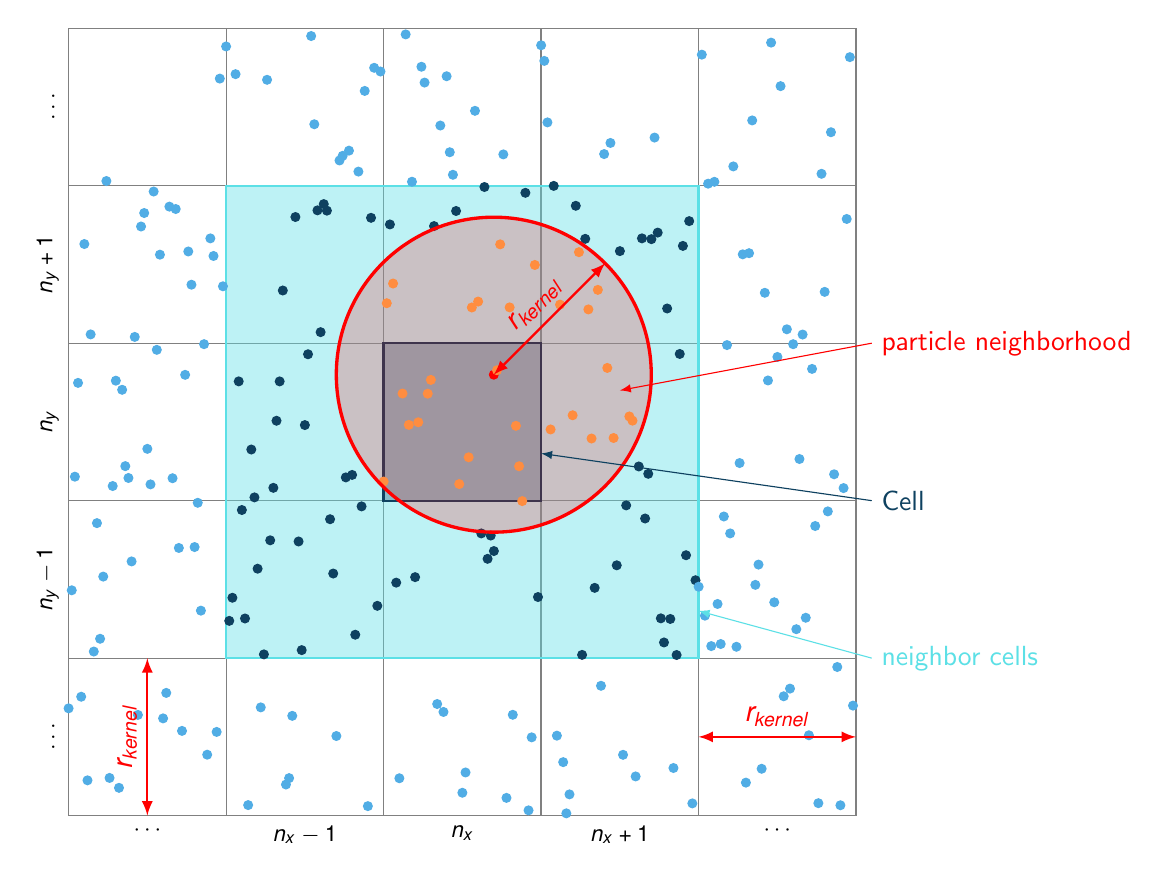
\begin{tikzpicture}[
    scale=2
 ]
\def\xMin{0}
\def\xMinSec{1}
\def\yMin{0}
\def\yMinSec{1}
\def\xMax{4}
\def\yMax{4}

\def\xxMin{-0.5}
\def\xxMinSec{0.5}
\def\yyMin{-0.5}
\def\yyMinSec{0.5}
\def\xxMax{4.5}
\def\yyMax{4.5}


\def\xpart{2.2}
\def\ypart{2.3}


\foreach \i in {\xxMin,\xxMinSec,...,\xxMax} {
        \draw [thin, gray] (\i,\yyMin) -- (\i,\yyMax);
    }
    \foreach \i in {\yyMin,\yyMinSec,...,\yyMax} {
        \draw [thin, gray] (\xxMin,\i) -- (\xxMax,\i);
    }


\draw (0,\yMin-0.5) node[below] {\footnotesize $\cdots$};
\draw (1,\yMin-0.5) node[below] {\footnotesize $n_x-1$};
\draw (2,\yMin-0.5) node[below] {\footnotesize $n_x$};
\draw (3,\yMin-0.5) node[below] {\footnotesize $n_x+1$};
\draw (4,\yMin-0.5) node[below] {\footnotesize $\cdots$};

\draw (\xMin-0.5,0) node[rotate = 90, above] {\footnotesize $\cdots$};
\draw (\xMin-0.5,1) node[rotate = 90, above] {\footnotesize $n_y-1$};
\draw (\xMin-0.5,2) node[rotate = 90, above] {\footnotesize $n_y$};
\draw (\xMin-0.5,3) node[rotate = 90, above] {\footnotesize $n_y+1$};
\draw (\xMin-0.5,4) node[rotate = 90, above] {\footnotesize $\cdots$};


\draw[color=AFLight, thick,fill=AFLight, fill opacity=0.4] (0.5,0.5) rectangle ++(3,3);
\draw[color=AFDark, thick, fill=AFDark, fill opacity=0.3] (1.5,1.5) rectangle ++(1,1);

\draw [color=red] plot [only marks, mark size=0.8, mark=*] coordinates {(\xpart,\ypart)};

\foreach \i in {-0.5,-0.48,...,4.5} {
    \pgfmathsetmacro{\y}{rand*2.5+2)}
    \pgfmathsetmacro{\r}{(\i-\xpart)*(\i-\xpart)+(\y-\ypart)*(\y-\ypart)}

    \pgfmathsetmacro{\col}{ifthenelse(\r<1,"AFOppo",ifthenelse(\i<0.5,"AFMiddle",ifthenelse(\i>3.5,"AFMiddle",ifthenelse(\y<0.5,"AFMiddle",ifthenelse(\y>3.5,"AFMiddle","AFDark")))))}

        \draw [color=\col] plot [only marks, mark size=0.8, mark=*] coordinates {(\i, \y)};
    }

\draw[color=red, very thick, fill=red, fill opacity=0.2](\xpart,\ypart) circle (1);


\pgfmathsetmacro{\xxpart}{\xpart+0.707106781}
\pgfmathsetmacro{\yypart}{\ypart+0.707106781}
\draw[<->, thick, red] (\xpart,\ypart) -- (\xxpart,\yypart) node[midway, above, sloped] {$r_{kernel}$};


\draw[<->, thick, red] (3.5,0) -- (4.5,0) node[midway, above, sloped] {$r_{kernel}$};
\draw[<->, thick, red] (0,-0.5) -- (0,0.5) node[midway, above, sloped] {$r_{kernel}$};

\draw[->, AFDark] (4.6,1.5) node[right] {Cell} -- (2.5,1.8);

\draw[->, AFLight] (4.6,0.5) node[right] {neighbor cells} -- (3.5,0.8);

\draw[->, red] (4.6,2.5) node[right] {particle neighborhood} -- (3,2.2);

\end{tikzpicture}
\end{document}
